\documentclass[a4paper]{article}

\usepackage{natbib}
\usepackage[english]{babel}
\usepackage[utf8]{inputenc}
\usepackage{amsmath}
\usepackage{graphicx}
\usepackage[colorinlistoftodos]{todonotes}

\usepackage{tikz}
\usetikzlibrary{math,fpu,calc,fit,mindmap,backgrounds,positioning}

\usepackage{xspace}
\newcommand{\eg}{e.g.\xspace}
\newcommand{\etal}{et al.\xspace}
\newcommand{\ie}{i.e.\xspace}
\newcommand{\etc}{etc.\xspace}
\newcommand{\vs}{\textit{vs.}\xspace}

\title{From Social Attention to Social Modelling in Robotics:\\ The Robotic Social Awareness Model}

\author{Séverin Lemaignan}

\date{\today}

\begin{document}
\maketitle

\begin{abstract}

My current perspective could be summarized as:

1- mental representations are snapshots of what we are aware of;

2- awareness is the label we conveniently put on the process of attention;

3- attention at time t is the label we put on the set of the activated units in
a (biased) associative memory network;

4- modelling others’ mental representations is taking snapshots of their own
current state of awareness;

5- modelling other’s state of awareness, ie, their current attentional process,
is mediated by one’s own attentional system, typically through joint attention
mechanisms;

6- Points 1 to 5 essentially refer to a 'phenomenal' awareness (a 'raw' inner
experience). 'Phenomenal' awareness can be turned into 'access' consciousness
(the abstract, cognitive ability to reflect on the inner experience);

7- In robots, 'access consciousness' can be mapped to symbolic, logic
representations.

(2) is Graziano's Attention Schemata Theory; (3) is based on Biased Competition
Model of Attention, Desimone and Duncan 1995; (6) comes from Block 1996.

As you hopefully see, this drafts a sub-symbolic/symbolic hybrid model of
cognition that puts (social) attention at the centre of social cognition.

Some of the main 'gaps' are:

- mental representations are likely not simply instantaneous 'snapshots' --
even though I could argue that they indirectly embed a notion of time and
history as they are snapshots of activated units in an associative memory
network;

- equating attention to a set of activated units in a memory network raises
questions regarding the nature of these units: physical entities? active
interaction modalities? ...? In particular, the right level of abstraction of
these units is not immediately clear: the spectrum is rather large, from raw
perceptual inputs 'à la Tony Morse' to high-level units like objects, joint
gazing, etc.

- the Biased Competition Model of Attention supports interesting bottom-up and
top-down biasing mechanisms: bottom-up is quite clear (if a unit is activated
longer/stronger, it biases the resulting attention to this unit. Top-down is
less clear (but also potentially very interesting as it closes the loop between
the sub-symbolic and symbolic models): how more abstract cognitive process can
influence the memory network to bias the attention process?

- the access to other's mental representations is mediated by one's own
attentional system: the consequences of this mediation are not immediately
clear

- I conveniently map the split between 'phenomenal consciousness' and 'access
consciousness' respectively to sub-symbolic and symbolic computational
structures. This need to be better evidenced, if only because the frontier
between phenomenal and access consciousness is all be clear (as pointed by
Graziano).

- It is not yet clear how the sub-symbolic and symbolic models of the different
agent co-exist: is each agent a different unit in the same associative network?
one associative memory per agent? what about the symbolic level?

Now, as we discussed many times, the model is of little interest if it does not
have some predictive power.

Here a few social behaviours that I would like a robot to exhibit if endowed
with such a model -- Not proper predictions, though.

- behavioural alignment -> surface alignment and/or global alignment -> the
original 'maze' task by Pickering and Garrod is certainly relevant here: every
time you play the same game with the same person, the interaction is more fluid
- ability to pass false-belief tasks, including non-physical, abstract ones, -
recursive awareness: being aware of being aware -- typically evidenced by being
able to describe/verbalize its own state of awareness - 'natural' turn-taking:
I 'just' know when it is my turn to act - 'natural' protodeclarative pointing:
I 'just' know when I really need to draw your attention on something

The word 'just' is clearly the key here: these capabilities should be natural
in the sense that they naturally follow from the model. 

\end{abstract}

%%%%%%%%%%%%%%%%%%%%%%%%%%%%%%%%%%%%%%%%%%%%%%%%%%%%%%%%%%%%%%%%%%%%%%%%%%%%
%%%%%%%%%%%%%%%%%%%%%%%%%%%%%%%%%%%%%%%%%%%%%%%%%%%%%%%%%%%%%%%%%%%%%%%%%%%%
%%%%%%%%%%%%%%%%%%%%%%%%%%%%%%%%%%%%%%%%%%%%%%%%%%%%%%%%%%%%%%%%%%%%%%%%%%%%
\section{What do we aim for?}

Human social dynamics rely upon the ability to effectively attribute beliefs,
goals and percepts to other people. This set of meta-representational abilities
shapes what is called a theory of mind (ToM) or the ability to mentalize, and
leads to mutual modelling: the reciprocal ability to establish a mental model of
the other. This lays at the core of human interactions: normal human social
interactions depend upon the recognition of other sensory perspectives, the
understanding of other mental states, and the recognition of complex non-verbal
cues of attention and emotional state. As such, adapting and transferring these
cognitive skills to social robots is an important research objective.


Understanding and predicting one's behaviour.

An integrated theory of social cognition, applicable to robots

A principled yet practical approach to social cognition for artificial intelligence


\subsection{Problem Statement}


Symbolic approaches to social cognition work by first building a mental model of the
interacting humans. This is typically done by a combination of 3D situation
assessment (the robot builds and update a semantic 3D model of its environment)
and visual perspective taking (based on the estimation of the pose of the human
head). This permits the computation of allocentric, and more importantly,
egocentric spatial relations between the spatial entities in the environment
(we call it \emph{social situation assessment}).

This geometric computations are then turned into symbolic representations,
typically using logical statements (embedded in logic
programming~\cite{tenorth2009knowrob} or ontologies~\cite{lemaignan2010oro}).

The robot creates and continuously updates one symbolic model per
agent~\cite{lemaignan2010oro}. These models are then used by other cognitive
processes (task planning, dialogue, task execution supervision) that are
designed to take advantage of the agents' knowledge models to produce
socially-aware behaviours: for example, the task planner may plan manipulation
task using only entities visible to the human~\cite{lallement2014hatp}, or the
dialogue manager may use the specific knowledge model of the speaker to
interpret the speech, avoiding grounding ambiguities that might otherwise
occur~\cite{lemaignan2011grounding}.

This works well as long as we limit ourselves to the manipulation of the results
of visual perspective taking. However, one intuitively recognizes that social
modelling goes indeed beyond computing what the human perceives or does not
perceive. This has been clearly recognized in developmental psychology, for
instance with Flavell's distinction between \emph{cognitive connections} on one
hand, and \emph{mental representations} on the other hand (we will come back to
Flavell's \emph{connection-representation} account in
section~\ref{connection-representation}). Now, if we are to model someone else's
mind beyond a naive geometric model of their perception, we indeed enter the
realm of \emph{representations}. What are they? How to access them? How to
represent and manipulate them? These three questions lay at the core of this
work, and as such we effectively take over the point we previously made
in~\cite{lemaignan2015mutual}:  we ultimately want to come up with a
meta-representational cognitive system to \emph{represents
representations} (including representations of \emph{false} beliefs or unknown
facts, \ie suppositions).

We must immediately clarify that, even though this goal may seem to pre-suppose
\emph{symbolic} meta-representations, this is not the case: at that stage, we do
not have evidence that a particular kind of computational structure may better
support the representation and manipulation of mental representations.

\subsection{What is not adequately solved by current techniques?}

[give concrete examples of social situations that are not easily achieveable
with current (symbolic or not) approaches]

[this examples should be turned into predictions for what our proposal should be
able to achieve]

\subsection{From Social Attention to Social Modelling}

The hypothesis that we hereafter develop and turn into a cognitive model is the
following: \textbf{mental representations are snapshots of awareness, awareness being
itself a label for the memory-mediated process of attention}.

This extends to social cognition: \textbf{modelling others' mental representations is
taking snapshots of their current state of awareness}. As we do not have direct
access to others' process of attention, it has to be mediated. We suggest that
\textbf{modelling other's state of awareness is mediated by one's own
attentional system, through joint attention mechanisms}.

This results in the following set of hypotheses:

\begin{itemize}
    \item \textbf{H1}: 
\end{itemize}


\subsection{Surface Alignment vs Deep Grounding}

Pickering and Garrod~\cite{pickering2006alignment} argue that mutual understanding
starts mostly with a \emph{superficial alignment} at the level of the linguistic
representations, due to priming mechanisms, and that this local alignment may --
in some cases -- lead to a \emph{global alignment} of the semantic level
(\emph{deep grounding}).  For these authors, the convergence in dialogue, and
even the repair of some misunderstandings, is explained by this mimetic behavior
more than by a monitoring of each other's knowledge:

\begin{quote}
[\ldots] interlocutors do
not need to monitor and develop full common ground as a regular, constant
part of routine conversation, as it would be unnecessary and far too costly.
Establishment of full common ground is, we argue, a specialized and
non-automatic process that is used primarily in times of difficulty (when
radical misalignment becomes apparent).~\citep[p.179]{pickering2006alignment}
\end{quote}


analysis of behavioural alignment between partners (via
metrics like the recently proposed \emph{Individual Motor
Signature}~\cite{slowinski2016dynamic})

\subsection{Theory of Mind}

We previously covered the state of the research on theory of mind in social
robotics~\cite{lemaignan2015mutual}.

In~\cite{scassellati2002theory}, Scassellati gave
an initial account of Leslie's and Baron-Cohen's respective models of the
emergence of a theory of mind (we discuss them below) from the perspective of
robotics, but reported implementation work was limited to simple perceptual
precursors (like face detection or color saliencies detection). Since then,
research in this field has been focused on applications relying on Flavell's
\emph{Level 1}~\cite{flavell1977development} perspective-taking, \ie
perspective-taking that only requires perceptual abilities (``\emph{I see (you do
not see the book)}''), and actually mostly limited to visual perception (relevant
work include Breazeal~\cite{breazeal2006using}, Trafton~\cite{Trafton2005} and
Ros~\cite{Ros2010}).

Based on perspective taking \emph{Level 1} alone, Breazeal
\etal\cite{breazeal2009embodied} and Warnier \etal\cite{warnier2012when}
successfully tackled the classical hallmark of theory of mind, the false belief
experiment (also known as the ``Sally and Anne'' experiment, introduced
by~\cite{wimmer1983beliefs}, original experimental setting
by~\cite{baron1985does}). They demonstrated complete human-robot interaction
scenarios where robots recognize and handle false belief situations in dyadic or
triadic interactions, and exhibit helping behaviours that account for the
missing/false beliefs of the human partners.

\cite{devin2016implemented}



%%%%%%%%%%%%%%%%%%%%%%%%%%%%%%%%%%%%%%%%%%%%%%%%%%%%%%%%%%%%%%%%%%%%%%%%%%%%
%%%%%%%%%%%%%%%%%%%%%%%%%%%%%%%%%%%%%%%%%%%%%%%%%%%%%%%%%%%%%%%%%%%%%%%%%%%%
%%%%%%%%%%%%%%%%%%%%%%%%%%%%%%%%%%%%%%%%%%%%%%%%%%%%%%%%%%%%%%%%%%%%%%%%%%%%
\section{Foundations of the Socio-cognitive Awareness for Robots}

\subsection{Connections vs. representations}
\label{connection-representation}

In~\cite{flavell1990developmental}, Flavell relates perspective taking
\emph{Level 1} to establishing \emph{cognitive connections} (I see, I hear, I
want, I like, I fear...), in contrast to perspective taking \emph{Level 2} that
relates to manipulating \emph{representations}.  This is exemplified by
\emph{appearance-reality} tasks, like the \emph{elephant mask} experiment
proposed in~\cite{flavell1990developmental}: 3-years old children are not able
to tell that an experimenter hidden behind a large elephant mask but who speaks
normally \emph{looks} like an elephant, \emph{sounds} like the experimenter, and
\emph{really is} the experimenter.  It appears that, while those children are
able to explicitly manipulate cognitive connections (they know for instance that
these are largely independent of each other and that they can evolve over time)
and know as well that their own connections are independent of those of other
people, they do not think that one concept can \emph{seriously} (\ie non
playfully) hold several, possibly conflicting, representations.


\subsection{Phenomenal \vs Access Consciousness}

Neuroscientist view: Block's proposal of two kind of consciousness~\cite{block1996can}:
\emph{phenomenal} consciousness as the raw inner experience; \emph{access}
consciousness as the more abstract, cognitive ability to think about and report
on those experiences.

Does this map to the traditional sub-symbolic/symbolic divide that we observe in
artificial intelligence, and in particular in robotics?

The \emph{phenomenal consciousness} would then be the immediate raw perceptual
inputs: video streams from cameras, readings for torque and force sensors, joint
positions, etc.

The \emph{access consciousness} would typically be the symbolic representation
of these inputs.


We must however keep in mind that there is likely no such rigid dichotomy
between phenomenal consciousness and access consciousness. It is rather a
continuum of processing~\citep[p.55]{graziano2013consciousness}

Recursivity of consciousness: if I'm looking at a green apple, my cognitive
machinery can decide and report that I'm aware of green. I can also be aware of
the deciding and aware of the reporting~\citep[p.55]{graziano2013consciousness}.

\subsection{The Attention Schema Theory}

Our approach draws form the \emph{Attention Schema Theory}, proposed by
Grazino~\cite{graziano2013consciousness}.

What awareness can do? ``the brain \emph{does} attention, but \emph{knows}
awareness'': as such, ``awareness can in principle be verbally reported''.



\subsection{Associative Memory Networks}


In particular, used for behavioural alignment

\subsection{Semantic Networks}

Ontologies and other Knowledge Representation and Reasoning systems.

%%%%%%%%%%%%%%%%%%%%%%%%%%%%%%%%%%%%%%%%%%%%%%%%%%%%%%%%%%%%%%%%%%%%%%%%%%%%
%%%%%%%%%%%%%%%%%%%%%%%%%%%%%%%%%%%%%%%%%%%%%%%%%%%%%%%%%%%%%%%%%%%%%%%%%%%%
%%%%%%%%%%%%%%%%%%%%%%%%%%%%%%%%%%%%%%%%%%%%%%%%%%%%%%%%%%%%%%%%%%%%%%%%%%%%

\section{The Robotic Social Awareness Model}

\subsection{Overview}

Associative Memory as an Informational Proxy for the Attention System


\begin{enumerate}
    \item Perceptual inputs feed in an associative memory

    \item the resulting set of pre-activated units is the current
        \emph{focus of attention} -- this step may require dimensionality
        reduction techniques

    \item According to the Attention Schema Theory, by \emph{explicitely}
        labelling the activated and pre-activated units as being attended, we
        make the robot \emph{aware} of the corresponding phenomenons.

    \item The labelling occurs by the mean of a symbolic association within a
        semantic network (ontology)

\end{enumerate}

\subsection{Attention}

Modelled as a \emph{Biased Competition Model of
Attention}~\cite{desimone1995neural}.
Implemented using a particular \emph{Associative Memory Network} with an
additional top-down biasing mechanism.

\subsubsection{Memory-mediated Attention}

\emph{Attention} is modelled as the set of activated units in an associative
memory network.


Interplay between multi-modal social cues on one hand, and priming of previously activated physical
entities (objects, agents) and 

Attention


\begin{figure}[h!]
    \centering
        \resizebox{0.7\linewidth}{!}{%
        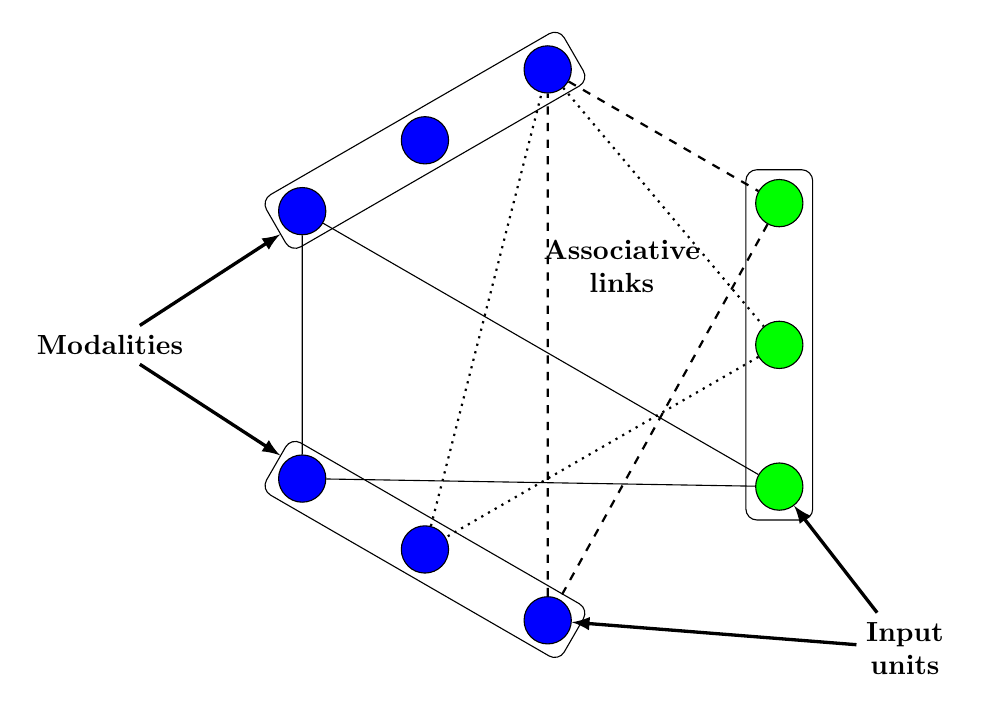
\begin{tikzpicture}[
                >=latex,
                every edge/.style={draw, very thick},
                every node/.style={font=\bf,align=center},
                input/.style={draw,circle, inner sep=0pt,minimum size=0.6cm}
            ]

            % draw the units
            \foreach \x [count=\xi] in {0, 120, 240}
                \foreach \y [count=\yi] in {-.6, 0, .6}
                    %\node[input, ball color=orange!\x!blue] at ($(\x:3)!\y!90:(0,0)$) (i\xi\yi) {};
                    \node[input, fill=blue!\x!green] at ($(\x:3)!\y!90:(0,0)$) (i\xi\yi) {};

            \node[draw,rounded corners, fit=(i11)(i12)(i13)] (modA) {};
            \node[draw,rounded corners, rotate fit=120,fit=(i21)(i22)(i23)] (modB) {};
            \node[draw,rounded corners, rotate fit=60,fit=(i31)(i32)(i33)] (modC) {};

            \node at (180:5.5) {Modalities} edge[->] (modB) edge[->] (modC);
            \node at (-40:6) {Input\\units} edge[->] (i13) edge[->] (i31);

            \path[draw,dashed, thick]  (i23) -- (i11) -- (i31) -- (i23);
            \path[draw,dotted, thick] (i23) -- (i12) -- (i32) -- (i23);
            \path[draw] (i21) -- (i13) -- (i33) -- (i21);

            \node at (1,1) {Associative\\links};
        \end{tikzpicture}
    }

    \caption{Associative Memory Network}
    \label{blabla}
\end{figure}



\subsubsection{Biasing Mechanisms}

Biasing competition~\cite{beck2009top}

The bottom-up biasing mechanism follows naturally from the structure of the
associatve memory model: a strong and long activation of a perceptual input
leads to the activation of the corresponding unit in the memory network and the
suppression of competing inputs.

The top-down mechanism is to be invented :-)
It should enable high-level decisional processes to effectively suppress (or
reinforce) units. The \emph{nature} and \emph{representation} of these
high-level processes is unclear, but might be of symbolic nature.



\subsection{Social Attention}

What do we call the \emph{attention state} of a partner?


Grazino~\cite{graziano2013consciousness}: ``the mental machinery to model
someone else attentional state is the same as the one used for oneself.''

``In both case, the purpose is understanding and predicting one's behaviour.''

Cues from which we reconstruct someone else's attentional state (from Graziano):
\begin{itemize}
    \item gaze direction
    \item facial expression
    \item body language
    \item prior knowledge of person
    \item location of salient objects
\end{itemize}

\subsection{What is the contribution, the novelty?}



%%%%%%%%%%%%%%%%%%%%%%%%%%%%%%%%%%%%%%%%%%%%%%%%%%%%%%%%%%%%%%%%%%%%%%%%%%%%
%%%%%%%%%%%%%%%%%%%%%%%%%%%%%%%%%%%%%%%%%%%%%%%%%%%%%%%%%%%%%%%%%%%%%%%%%%%%
%%%%%%%%%%%%%%%%%%%%%%%%%%%%%%%%%%%%%%%%%%%%%%%%%%%%%%%%%%%%%%%%%%%%%%%%%%%%
\section{What Does the Model Predict?}

\subsection{Protodeclarative pointing}

Protoimperative vs protodeclarative pointing~\cite{baron1986perceptual}

\subsection{Behavioural Alignment}
\subsection{Verbalization of the (Social) Attentional Process}
\subsection{False-beliefs}


Picture ordering protocol, with \emph{mechanical}, \emph{behavioural} and
\emph{intentional} sequences~\cite{baron1986mechanical}

\subsection{Symbol Grounding}

\subsection{Recursive Awareness}

I can describe what I'm aware of, I can also recursively be aware I'm describing
my state of awareness, and I can verbalize this second order awareness.

This should work \emph{Attention Schema} theory because the attention schema
is seen as a regular sensory
representation~\citep[p.55]{graziano2013consciousness}.

\subsection{Adapted behaviour to the interacting agent}

A robot facing a baby, a 3 years old, a 5 years old, a 13 years old or an adult
should behave differently.

%%%%%%%%%%%%%%%%%%%%%%%%%%%%%%%%%%%%%%%%%%%%%%%%%%%%%%%%%%%%%%%%%%%%%%%%%%%%
%%%%%%%%%%%%%%%%%%%%%%%%%%%%%%%%%%%%%%%%%%%%%%%%%%%%%%%%%%%%%%%%%%%%%%%%%%%%
%%%%%%%%%%%%%%%%%%%%%%%%%%%%%%%%%%%%%%%%%%%%%%%%%%%%%%%%%%%%%%%%%%%%%%%%%%%%
\section{The Functional Pre-Requisites for Social Robots}

\subsection{Social Assessment}

\subsubsection{Gaze Direction}
\subsubsection{Facial and Body Expressions}
\subsubsection{Gestures}

\subsection{Situation Assessment}

Including saliency information

%%%%%%%%%%%%%%%%%%%%%%%%%%%%%%%%%%%%%%%%%%%%%%%%%%%%%%%%%%%%%%%%%%%%%%%%%%%%
%%%%%%%%%%%%%%%%%%%%%%%%%%%%%%%%%%%%%%%%%%%%%%%%%%%%%%%%%%%%%%%%%%%%%%%%%%%%
%%%%%%%%%%%%%%%%%%%%%%%%%%%%%%%%%%%%%%%%%%%%%%%%%%%%%%%%%%%%%%%%%%%%%%%%%%%%
\section{Evaluation of the Model}

\subsection{Does it perform as well as Symbolic Architectures?}
\subsection{Comparison with Symbolic Situation Assessment}




\bibliographystyle{plain}
\bibliography{biblio}

\end{document}
